\documentclass[12pt,twoside]{article}

%\usepackage{amsthm}%
\usepackage{amsmath}
\usepackage{amssymb}
\usepackage{amsfonts}
\usepackage[margin=1in]{geometry}
\usepackage{enumerate}
\usepackage{verbatim}
\usepackage{graphicx}
\usepackage{hyperref}


\newenvironment{proof}{\noindent{\bf Proof:} \hspace*{1mm}}{
	\hspace*{\fill} $\Box$ }
\newenvironment{proof_of}[1]{\noindent {\bf Proof of #1:}
	\hspace*{1mm}}{\hspace*{\fill} $\Box$ }
\newenvironment{proof_claim}{\begin{quotation} \noindent}{
	\hspace*{\fill} $\diamond$ \end{quotation}}

\newtheorem{thm}{Theorem}
\newtheorem{lemma}[thm]{Lemma}

\newcommand{\mbf}{\mathbf}
\newcommand{\mrm}{\mathrm}

\newenvironment{centered}[0]{%
  \begin{list}{}{%
    \setlength{\topsep}{0pt}%
    \setlength{\leftmargin}{.25in}%
    \setlength{\rightmargin}{.25in}%
    \setlength{\listparindent}{\parindent}%
    \setlength{\itemindent}{\parindent}%
    \setlength{\parsep}{\parskip}%
  }
  \item[]}{\end{list}}
\newcommand\abs[1]{\left|#1\right|}
\newcommand\given[1][]{\:#1\vert\:}
\newcommand{\legendre}[2]{\genfrac{(}{)}{}{}{#1}{#2}}
\setcounter{tocdepth}{1}
\newtheorem{theorem}{Theorem}



\title{Constructing Pairing-Friendly Elliptic Curves }
\date{\today}
\author{ Peter Manohar, Xingyou Song} 

\begin{document}

\maketitle

\abstract{The goal of this report is to....
}

\tableofcontents

\section{Introduction}

In this section, we shall define key concepts needed for our report. We will prove some of the more important results, and cite a source otherwise.

\subsection{Elliptic Curves} 
For our project, we shall define an elliptic curve to be a curve of the form:
\begin{equation}
E: \ y^2 = x^3 + Ax + B 
\end{equation}
where $A$ and $B$ are elements of some field $\mathbb F$, with char$(\mathbb F) \ne 2,3$. The curve $E$ is nonsingular if $\frac{\partial F}{\partial x}$ and $\frac{\partial F}{\partial y}$ are not simultaneously $0$ for all points on $E$. It follows that $E$ is nonsingular $\iff x^3+ Ax+ B$ has distinct roots. Through Vieta's formulas, $E$ has distinct roots $\iff ((r_{1} - r_{2})(r_{1} - r_{3})(r_{2} - r_{3}))^{2} = -(4A^{3} + 27B^{2})$ is nonzero. Therefore, we shall also require that the discriminant of $E$,
\begin{equation} 
\Delta = -16(4A^{3} + 27B^{2})
\end{equation}
is nonzero. 
The j-invariant of $E$ is defined by:
\begin{equation}
j(E) = 1728 \frac{4A^{3}}{4A^{3} + 27B^{2}}
\end{equation}
\subsection{Group Law} 
The points on an elliptic curve form an additive abelian group. We shall define the group law geometrically. \\
Let $P = (x_p, y_p), Q = (x_q, y_q)$. A line through $P$ and $Q$ intersects $E$ at a third point, $R = (x_r,y_r)$. We define $P + Q := (x_r,-y_r)$. Pictorally, this looks like \\
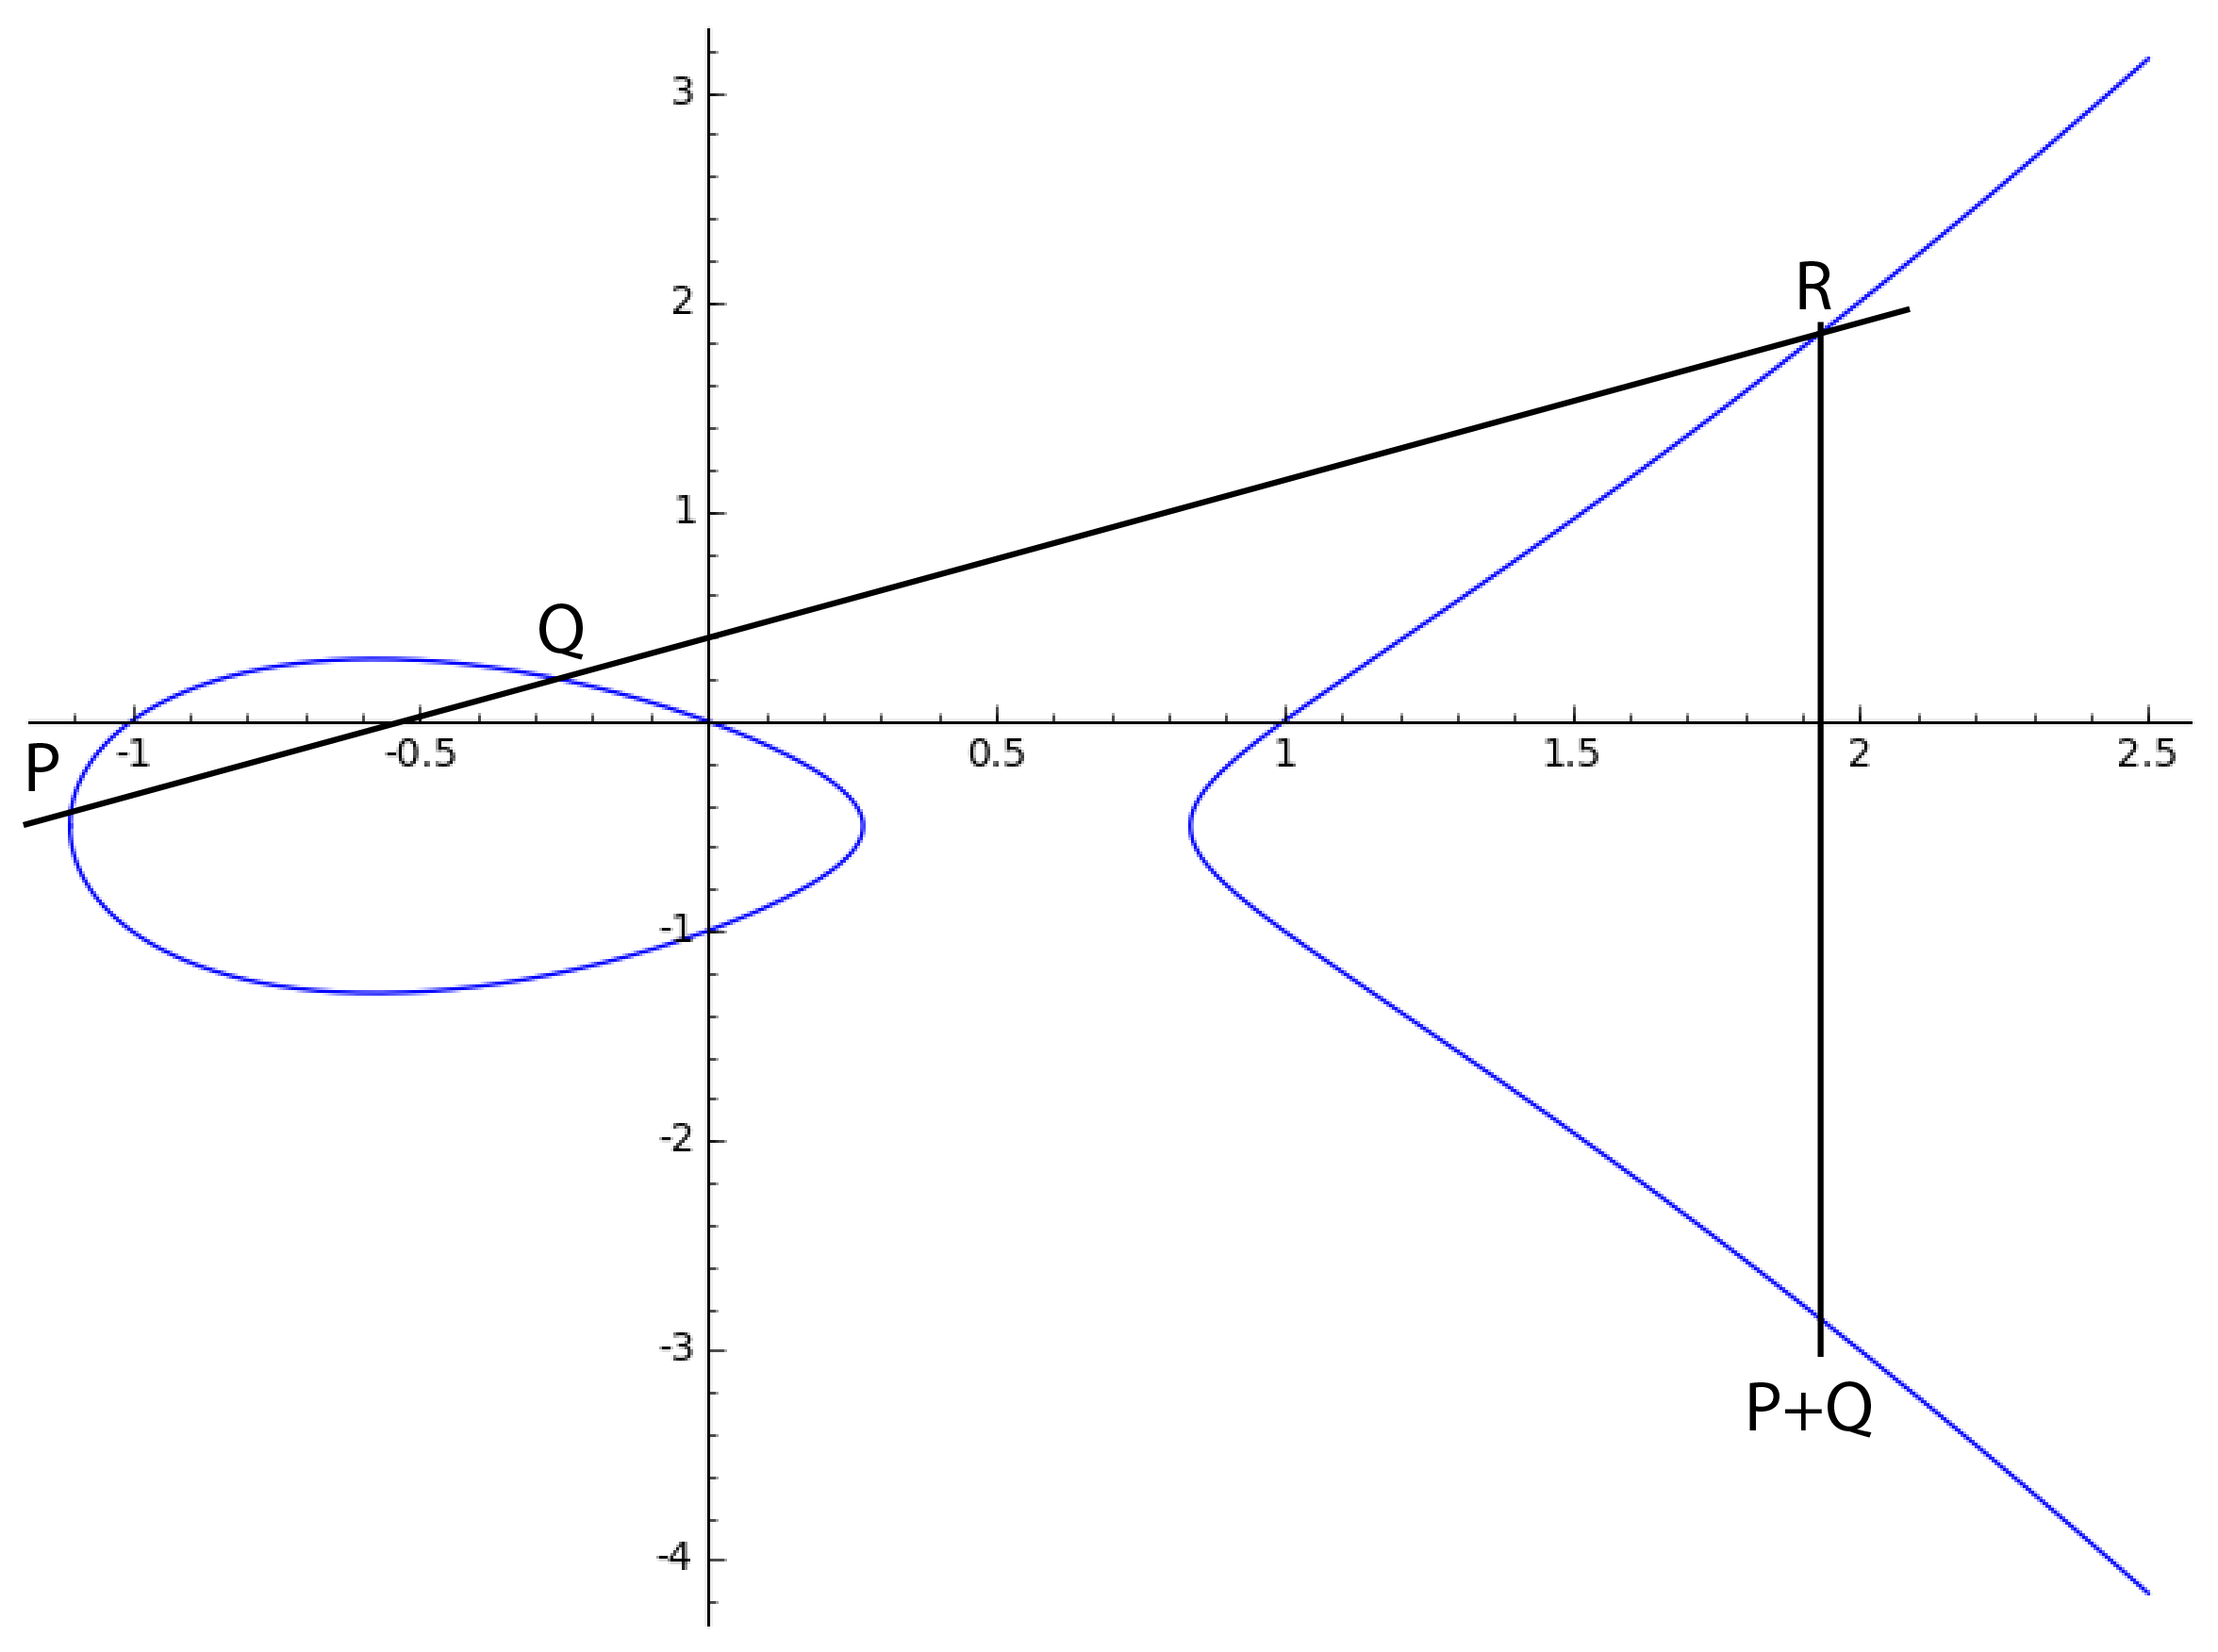
\includegraphics[width=6in]{grouplaw.png}
The group law can also be defined in terms of algebraic formulas, which can be found in [1]. %[1] is silverman%

\subsection{Notation}
\begin{itemize}
\item $\mathbb F$ is a field
\item $\overline{\mathbb F}$ is the algebraic closure of $\mathbb F$
\item $\mathbb F_p$ is a field with $p$ elements, where $p$ is prime
\item $E(\mathbb F) = \{\mathbb F \times \mathbb F \given E(x,y) = 0\}$
\item $\phi$ is an isogeny (or endomorphism)
\item $\phi_p$ is the Frobenius endomorphism
\end{itemize}



\subsection{Isogenies} 
An isogeny of two elliptic curves $E_1$ and $E_2$ defined over a field $\mathbb F$ is a nonconstant morphism $\phi: E_1 \to E_2$, where $\phi$ is a group homomorphism from $E_1(\overline{\mathbb F}) \to E_2(\overline{\mathbb F})$. $E_1$ and $E_2$ are isomorphic if $\exists \phi_1: E_1 \to E_2$ and $\phi_2: E_2 \to E_1$, isogenies, such that $\phi_2 \circ \phi_1 =  $ Identity.

\subsubsection{Separable and Inseparable Isogenies}
Any isogeny $\phi$ can be expressed as $\phi(x,y) = (\frac{u(x)}{v(x)}, \frac{s(x)}{t(x)}y)$, where $u,v,s,t \in \mathbb F[x]$, and $\gcd(u,v) = \gcd(s,t) = 1$. [3] %[3] is mit reference
An isogeny is separable if $(\frac{u}{v})' = 0$, and is inseparable otherwise. The degree of an isogeny is defined as $\deg(\phi) := \max(\deg(u), \deg(v))$. [3]
For any separable isogeny $\phi$, $\deg(\phi) = \abs{ \ker \phi}$.

\subsubsection{Dual isogenies}
\begin{theorem}
Let $\phi: E_1 \to E_2$ be an isogeny. Then $\exists$ a unique $\hat{\phi}: E_2 \to E_1$ such that $\hat \phi \circ \phi = [n]$, where $n = \deg(\phi)$.
\end{theorem}
\noindent The proof of this can be found in either [1] or [3]. Furthermore, for any two isogenies $\phi_1$ and $\phi_2$, $\widehat{\phi_1 + \phi_2} = \hat \phi_1 + \hat \phi_2$.
\subsection{Endomorphisms}

An endomorphism is an isogeny from $E$ to itself. The endomorphisms of $E$ form a ring, where addition is addition of functions and multiplication is function composition.

\subsubsection{Examples}

The map $[n]: E \to E$, where $[n]P = P + P + \dots + P$ ($n$ times) is an endomorphism.
\\ \\
\noindent If $E$ is defined over $\mathbb F_p$, the Frobenius map $\phi_p: E \to E$ defined by $\phi_p(x,y) := (x^p, y^p)$ is an (inseparable) endomorphism.

\subsubsection{Trace of an Endomorphism}

\begin{theorem}
For any endomorphism $\phi$, $\phi + \hat \phi = 1 + \deg(\phi) - \deg(1-\phi)$, where we can regard the RHS as an endomorphism by the map $n \mapsto [n]$.
\end{theorem}
\begin{proof}
As endomorphisms, 
\begin{flalign*}
& [\deg(1-\phi)] = \widehat{(1-\phi)}(1-\phi) = (\hat 1 - \hat \phi)(1-\phi) = (1 - \hat \phi)(1-\phi) \\
&= 1 - \hat \phi - \phi + \hat \phi \circ \phi = 1 - \hat \phi - \phi + [\deg(\phi)] \\
& \implies \phi + \hat \phi = 1+ [\deg(\phi)] - [\deg(1- \phi)] 
\end{flalign*}
\end{proof}
\\
By the above theorem, we can now define trace$(\phi) := \phi + \hat \phi$.
\begin{theorem}
$\#E(\mathbb F_p) = p + 1 - t$, where $t = {\rm trace}(\phi_p)$
\end{theorem}
\begin{proof}
The fixed field of $\phi_p$ is $\mathbb F_p$, and $1- \phi_p$ is separable (see [3]). Therefore, $\ker(1- \phi_p) = \#E(\mathbb F_p)$. It is clear that $\deg(\phi_p) = p$ by definition ($u(x) = x^p$ and $v(x) = 1$). We have that
\begin{flalign*}
&\ker(1-\phi_p) = \deg(1-\phi_p) = 1 + \deg(\phi_p) - {\rm trace}(\phi_p) = p + 1 - t \\
&\implies \#E(\mathbb F_p) = p + 1 -t
\end{flalign*}
\end{proof}


\bigskip


\begin{theorem} 
If $K$ is a field of characteristic $0$ or does not divide $m$, then
$ E[m] \simeq Z_{m} \oplus Z_{m}$.  
\end{theorem} 
The proof of this is mainly using the fundamental theorem of abelian groups, and analyzing the decomposition of the torsion group (TODO?) 



\subsection{j-invariant} 

\begin{theorem}
Two elliptic curves $E_1(\mathbb F)$ and $E_2(\mathbb F)$ are isomorphic over $\overline{\mathbb F} \iff j(E_1) = j(E_2)$. Furthermore, $\forall j_0 \in \overline{\mathbb F}$, $\exists$ an elliptic curve $E(\mathbb F)$ such that $j(E) = j_0$.
\end{theorem}
The proof requires some lengthy algebraic manipulation, which can be found in [1]. As a consequence of the proof, for any $j \in \overline{\mathbb F}$, we can define an canonical elliptic curve $E$ associated with this j-invariant. We see that 

  
\begin{flalign*} 
& E: y^{2}  = x^{3} + \frac{3j}{1728 - j}x + \frac{2j}{1728 - j} \text{\ if \ } j \ne 0, 1728\\
& E: y^2 = x^3 + 1 \text{\ if \ }  j = 0 \\
& E: y^2 = x^3 + x \text{\ if \ } j = 1728
\end{flalign*}

\begin{comment}
A question arises when two elliptic curves over a field $E_{1}(K), E_{2}(K)$ are have a bijective isogeny, i.e. are isomorphic with respect to the group law. 
An intuitive answer is that the points on elliptic curves be transformed algebraically, which will use different Weierstrass Equations

Note the transformation  

\begin{align*}
x' = \mu^{2}x \\   
y' = \mu^{3}y 
\end{align*}

implies, after plugging into the Weierstrass equation,

\begin{equation} 
(y')^{2} = (x')^{3} + \mu^{4}Ax' +\mu^{6}B \implies (y')^{2} = (x')^{3} + A'x' + B'  
\end{equation} 
where $A' = \mu^{4}A, B' = \mu_{6}B$. $\mu$ may not exist in the field $K$, but only in its closure $\bar{K}$. 

From here, we define the j-invariant $j$ of a Weierstrass Form to be 
\begin{equation} 
j(E) = 1728 \frac{4A^{3}}{4A^{3} + 27B^{2}}
\end{equation}

Note that the $j$ invariant is homogenous; scalings of the form from (5) will still leave $j$ constant. Given a $j$, then the canonical elliptic curve associated with this j-invariant will be 
\end{comment}

\subsubsection{Example}
$E_1(\mathbb F)$ and $E_2(\mathbb F)$ can be isomorphic over $\overline{\mathbb F}$, but not over $\mathbb F$. As an example, consider the curves $E_1: y^{2} = x^{3} - 25x$, $E_2: y^{2} = x^{3} - 4x$ have $j=1728$. $\#E_1(\mathbb Q) = \infty$, but $\#E_2(\mathbb Q) < \infty$. The transformation $(x,y) \rightarrow (\mu^{2}x, \mu^{3}y)$, $\mu = \frac{\sqrt{10}}{2}$ establishes an isomorphism over $\mathbb Q(\sqrt{10})$, but no such isomorphism exists over $\mathbb Q$.

From this example, we can see that we do not necessarily need the full closure $\overline{\mathbb F}$; we only needed $d \in \mathbb F$ such that $d= \mu^{2}$, which in this case was $\mathbb Q(\sqrt{10})$.

\subsection{Twists} 
Two curves $E_1(\mathbb F)$ and $E_2(\mathbb F)$ are {\it twists} if they are isomorphic over $\overline{\mathbb F}$ but not over $\mathbb F$.
\subsubsection{Quadratic Twists}
In particular, we are interested in quadratic twists. If $E: y^2 = x^3 + Ax+ B$ is an elliptic curve defined over $\mathbb F$, and $d \in \mathbb F$ is a nonsquare, then we define the {\it quadratic twist of E} as $\tilde E: y^2 = x^3 + d^2Ax + d^3B$.

\begin{theorem}
If $E: y^2 = x^3 + Ax + B$ is an elliptic curve over $\mathbb F_p$ with $\#E(\mathbb F_p) = p+ 1 - t$, then $\#\tilde E(\mathbb F_p) = p+ 1 + t$
\end{theorem}
\begin{proof}
Let $\legendre{\cdot}{p}$ be the legendre symbol mod $p$. For any $x \in \mathbb F_p$, we see that $1 + \legendre{x^3+Ax+B}{p} = $ \# of points on $E$ with x-coordinate $x$. Therefore, 
\begin{flalign*}
\#E(\mathbb F_p) = 1 + \sum_{x \in \mathbb F_p} {(1 + \legendre{x^3+Ax+B}{p})} = p + 1 + \sum_{x \in \mathbb F_p} {\legendre{x^3+Ax+B}{p}}
\end{flalign*}
Since $\mathbb F_p$ is a field, $\forall x \in \mathbb F_p$, $\exists x' \in \mathbb F_p$ such that $d x' = x$. Therefore, for $\tilde E(\mathbb F_p$, we have that
\begin{flalign*}
&\#\tilde E(\mathbb F_p) = 1 + \sum_{x \in \mathbb F_p} {(1 + \legendre{(dx)^3+A(dx)+B}{p})} = p + 1 + \sum_{x \in \mathbb F_p} {\legendre{d^3(x^3+Ax+B)}{p}} \\
& = p + 1 + \sum_{x \in \mathbb F_p} {\legendre{d}{p} \legendre{d^2}{p} \legendre{x^3+Ax+B}{p}} = p + 1 - \sum_{x \in \mathbb F_p} {\legendre{x^3+Ax+B}{p}}
\end{flalign*}
\end{proof}

\subsection{The Complex Lattice}
\begin{theorem} 
Let $\omega_{1}, \omega_{2}$ be linearly independent points in $C$. Then define the lattice 
$$ L = Z\omega_{1} + Z \omega_{2}$$ Then there exists an elliptic curve that is isomorphic to $C/ L$. 
\end{theorem}
Define $G_{k}(L) = \sum_{\omega \in L}\omega^{-k}$. Then define the Weierstrass $\wp (z) $ function as follows: 

\begin{equation} 
\wp(z) = \frac{1}{z^{2}} + \sum_{\omega \in L}\left(\frac{1}{(z-\omega)^{2}} - \frac{1}{\omega^{2}}\right) 
\end{equation}  
Then this function can easily be shown, by applications of complex analysis, to be convergent and meromorphic, as well as periodic. Then the derivative $\wp(z)$ is 
\begin{equation} 
\wp ' (z) = -2 \sum_{\omega \in L} \frac{1}{(z- \omega)^{2}} 
\end{equation} 

Now we have a isomorphism from the additive group on $C/L$ to the the group of elliptic points on $E(C)$, by the map $$z \rightarrow ( \wp(z), \wp' (z)), \> \> \> \> \> 0 \rightarrow O $$ with $E$ being defined as 
\begin{equation} 
E: y^{2} = 4x^{3} - g_{2}x - g_{3} 
\end{equation} 
where $g_{2} = 60_{4}, g_{3} = 140G_{6}$  
Note that the periodicity will give: 

\begin{equation} 
(\wp(z_{1}), \wp'(z_{1})) \oplus (\wp(z_{2}), \wp'(z_{2})) = (\wp(z_{1} + z_{2}), \wp'(z_{1} + z_{2})) 
\end{equation} which gives rise to the corresponding group law on elliptic curves. 

Now we relate the $j$-invariant on curves to the $j-$function of a complex lattice. First, let rescale our lattice $L$ to $Z\tau + Z$ where $\tau = \frac{w_{1}}{w_{2}}$. First, define $q = e^{2\pi \i \tau}$. Then the j-invariant related to the lattice parameter is 
\begin{equation}
j(\tau) = 1728 \frac{g_{2}^{3}}{g_{2}^{3} - 27 g_{3}^{2}} 
\end{equation} 
 
 
The proof of all of this we won't go into detail in this paper, but this gives rise to the relationship between the complex lattice and isogenies, mainly integer endomorphisms $[m]$ give rise to $ z \rightarrow mz$, and for multiplication by a complex number $c$, we have $z \rightarrow cz$, which will induce a endormorphism on the corresponding elliptic curve.   


For curves defined on a field $K$, there is a homomorphism $K \rightarrow C$ if we linearly map the finite basis elements of $K$, $\alpha_{1}, ...,\alpha_{n}$ respectively to any algebraically independent set of elements in $C$, $\tau_{1},..., \tau_{n}$, so we can regard $E(K)$ as a curve in $C$.  

\subsubsection{Using Quadratic Lattices }
Consider the case when our lattice $L = O_{D}$ for some discriminant $D$, where the basis elements will be $[1, \sqrt{D}/2] $ or $[1, \sqrt{D}]$ depending on $D$ is $1, 3 (\mod 4)$ (????? casework) 

Then define the Hilbert Class polynomial $H_{D} \in Z[X]$ that is the minimal polynomial that contains the $j(L)$ as a root. There are many ways to calculate this, but we won't get to that in this paper. Thus, we can define an elliptic curve based on a square free discriminant $D$.  

\subsection{Pairings}
Then the Weil-Pairing $e_{r}$ is defined as a bilinear map,  

\begin{equation} 
e_{r}: E[r] \times E[r] \rightarrow \mu_{r}
\end{equation} where $\mu_{r}$ is the set of primitive roots of unity in $\bar{K}$, i.e. $\mu_{r} = \{x | x^{r} =1 \}$. In other words, instead of working with the $r$-torsion group of $E(K)$, we may work with the much simpler objects in the extension field of $K$. \\ 

Then we may define the embedding degree to be the degree of the extension field $K(\mu_{r})$, or in other words, $[K(\mu_{r}): K]$. It is shown that then, if $k$ is the embedding degree with respect to $r$, then $k$ is the smallest integer such that $r$ divides $q^{k} -1$. 
 


\section{Motivations and Applications} 

\subsection{Discrete Log Problem}
In the discrete log problem, we are given any group $G$, with a base generator element $P$, with a ciphertext $Q$, where the problem involves finding $k$ such that $P^{k} = Q$ in $G$. \\ \\
For elliptic curves, this becomes using a base point $P$ with high degree, in a finite field $F_{p}$. However, note that by the theorem of finite abelian groups, the elliptic curve group is isomorphic to ------------

\subsubsection{Pohlig-Hellman Attack}
For an element $P$, assume it has order $N$ in the group $G$. Then the prime factorization of $N$, is important to the adversary; i.e. if 
$$ N = \prod_{i}q_{i}^{e_{i}} $$ then if we need to find $k$ such that $P^{k} = Q$, then all we need to do is find $k$ in its base $q_{1}, q_{2},...$ expansions and then construct $k$ using the Chinese Remainder Method. We can do so on each $q_{i}$ by successively iteration. Thus the difficulty of attacking this problem relies on the largest prime dividing $N$. TODO(too long) \\ 

This implies that we will need to find elliptic curves that have large- prime order torsion groups




\section{Generating Curves} 

\subsection{CM Method} 
The general method of generating curves is the CM - method. 
The method involves, given $(p, N)$,  take $t = p+1 - N$, with $4p = t^{2} + s^{2}|D|$, where $D$ is square free. Then compute the Hilbert class polynomial $H_{D}(X)$, and find $j$ such that $H_{D}(j) = 0 \mod p$. Using (9), we can then construct the explicit formula of the curve.   










\bibliographystyle{alpha} 
\bibliography{references}
[1]. silverman
[2]. washington
[3]. mit
\end{document}